\documentclass[journal,twocolumn]{IEEEtran}
\usepackage[utf8]{inputenc}
\usepackage[T5]{fontenc}
\usepackage[vietnamese,english]{babel}
\usepackage{amsmath,amssymb,amsfonts}
\usepackage{algorithmic}
\usepackage{graphicx}
\usepackage{textcomp}
\usepackage{booktabs}
\usepackage{hyperref}
\usepackage{multirow}
\usepackage{array}
\usepackage{float}
\usepackage{makecell}
\usepackage{tabularx}

\begin{document}

\title{A Two-Stage Framework for Urban Traffic Management: From Camera-Level Vehicle Estimation to Temporal Attention-Guided Spatio-Temporal Graph Forecasting}

\author{Viet-Anh~Le
\thanks{Viet-Anh Le is with the Posts and Telecommunications Institute of Technology (PTIT), Vietnam (e-mail: anhlv.b23kh002@stu.ptit.edu.vn).}%
}

\maketitle

\begin{abstract}
Urban traffic congestion presents major operational and socio-economic challenges in modern metropolises. While surveillance camera networks offer accessible, high-coverage visual feeds, transforming raw video streams into reliable network-wide traffic forecasts requires solving two coupled sub-problems: (1) camera-level visual vehicle count estimation, and (2) network-wide multi-horizon traffic flow forecasting. In this paper, we present a unified framework integrating visual perception and spatio-temporal graph modeling over a real-world urban road network in Ho Chi Minh City, Vietnam. For Sub-problem 1, a ConvNeXt-Tiny backbone with a direct regression head estimates continuous counts of cars and motorbikes directly from camera feeds (trained on 4,000 images, validated on 1,000, and tested on 1,000 images). For Sub-problem 2, we construct a 608-node directed traffic graph $\mathcal{G}=(\mathcal{V}, \mathcal{E}, W)$ built from Ho Chi Minh City Traffic Portal cameras with RBF-weighted road distances. Addressing the fundamental flaws of single-node independent forecasting—which ignores dynamic traffic spillover—we introduce \emph{TA-STGCN} (Temporal Attention-Guided Spatio-Temporal Graph Convolutional Network), an architecture coupling Chebyshev Spectral Graph Convolutions ($K=3$), 1D Gated Temporal Convolutions (GLU), and Model-Level Multi-Head Temporal Self-Attention. Comprehensive evaluations across 5 independent random seeds ($42, 100, 2024, 777, 999$) demonstrate that TA-STGCN achieves superior multi-step forecasting accuracy ($\text{MAE} = 3.1923 \pm 0.0112$, $\text{RMSE} = 4.3435 \pm 0.0142$) across 6 forecast horizons ($t+1$ to $t+6$, 5-to-30 minutes ahead), outperforming traditional GCN-LSTM and standard STGCN baselines while maintaining a significantly lower parameter footprint (165,318 parameters vs. 364,198 for GCN-LSTM and 303,846 for STGCN).
\end{abstract}

\begin{IEEEkeywords}
Intelligent Transportation Systems, Urban Traffic Forecasting, ConvNeXt-Tiny Direct Regression, TA-STGCN, Temporal Attention, Spatio-Temporal Graph Neural Networks.
\end{IEEEkeywords}

\section{Introduction}

\subsection{Background and Motivation}
Rapid global urbanization and the exponential growth of personal motor vehicles—particularly passenger cars and motorcycles—have led to severe urban traffic congestion in developing metropolises, such as Ho Chi Minh City, Vietnam. Constructing new physical road infrastructure requires substantial financial capital and extended timeframes, offering minimal immediate relief. Consequently, Intelligent Transportation Systems (ITS) powered by Artificial Intelligence (AI) have become an essential, cost-effective strategy for real-time traffic perception, adaptive signal control, and proactive congestion forecasting.

Figure~\ref{fig:traffic_jam} illustrates a representative urban traffic congestion scene in Ho Chi Minh City, highlighting extreme vehicle density and complex occlusions between passenger cars and motorcycles.

\begin{figure}[htbp]
\centering
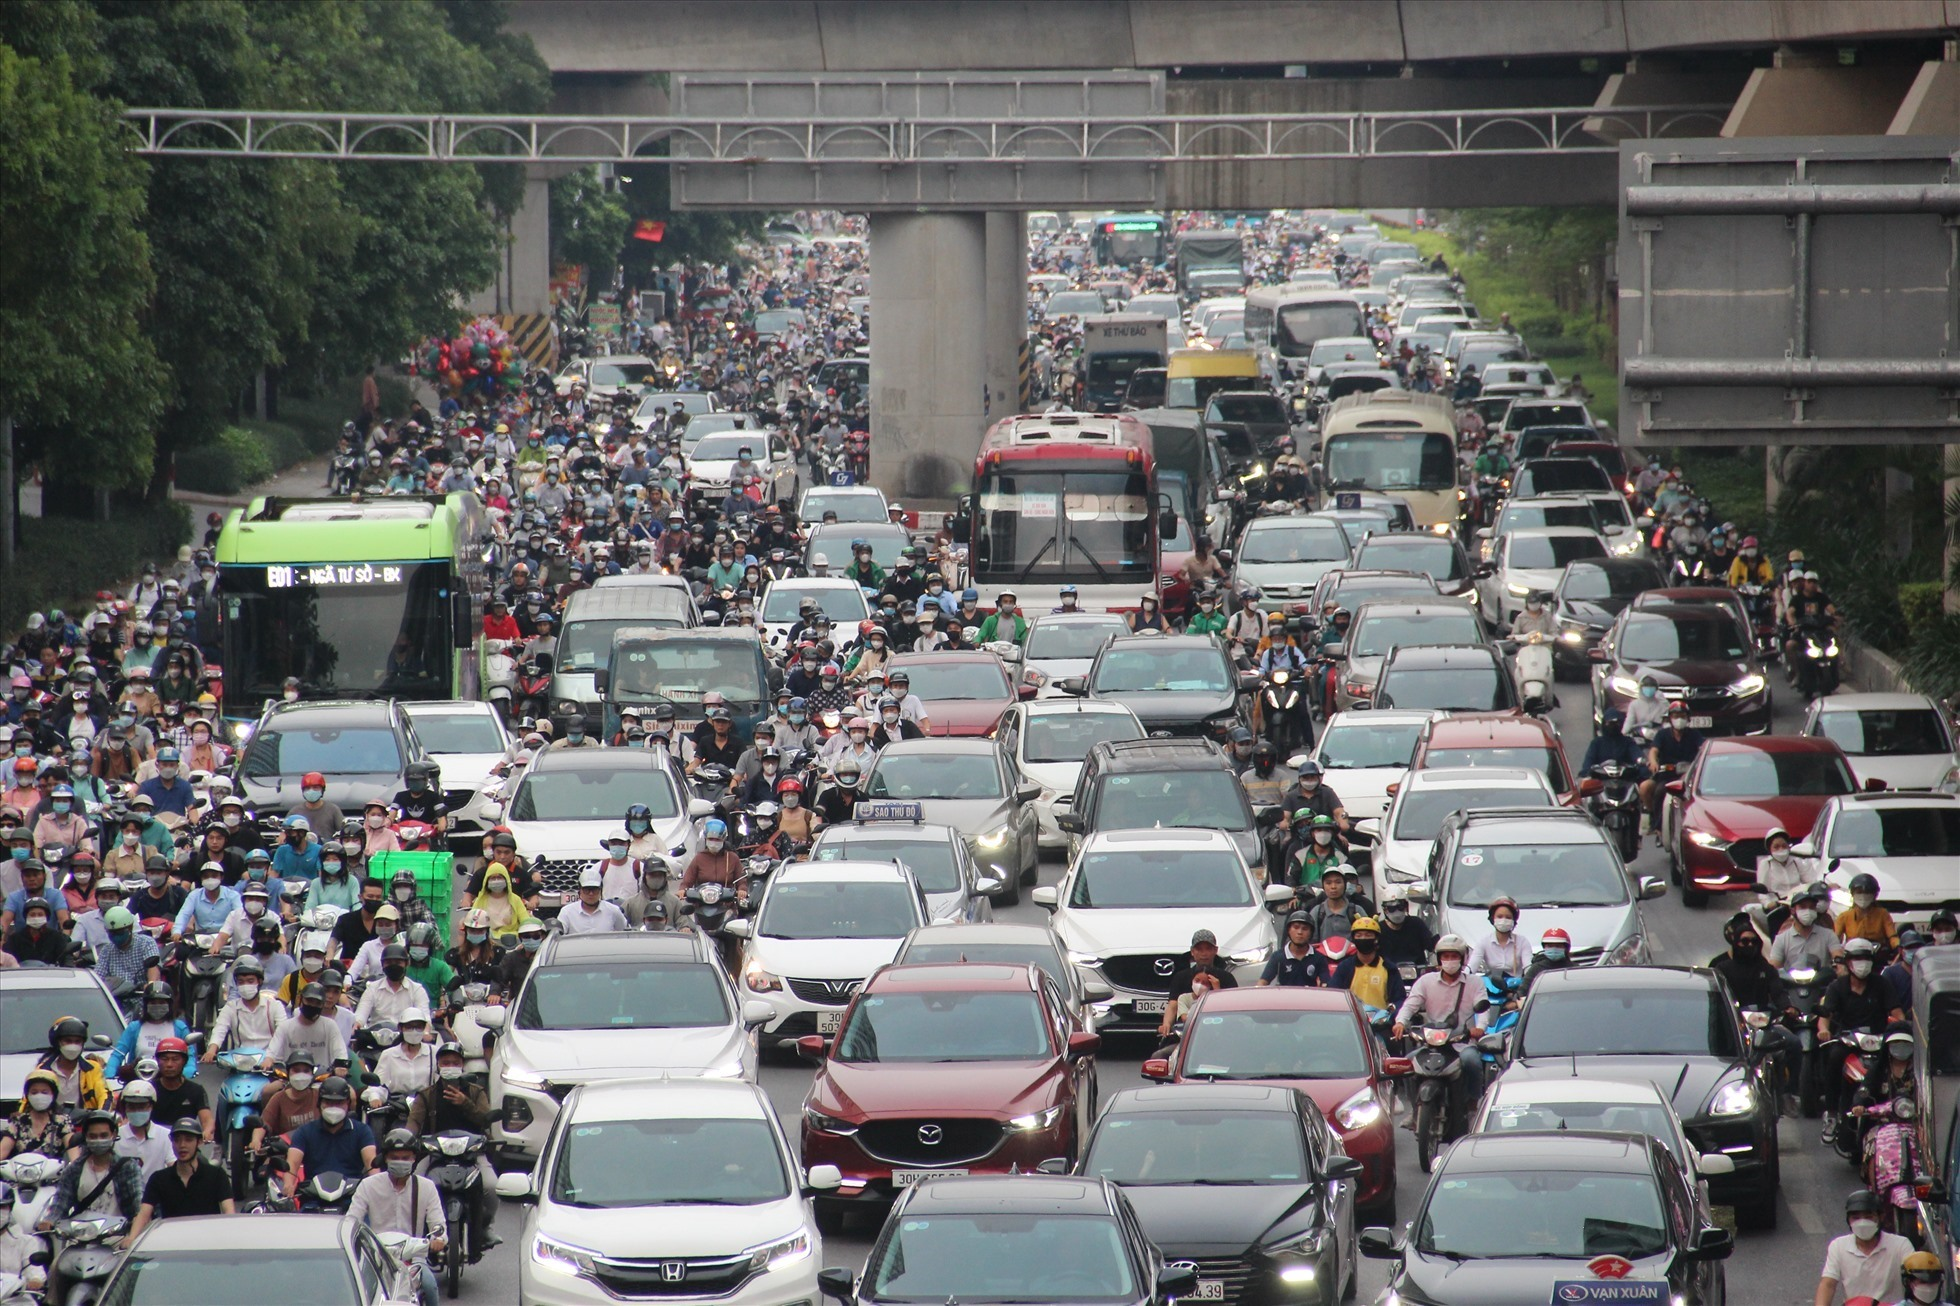
\includegraphics[width=\columnwidth]{fig/traffic_jam.jpg}
\caption{Urban traffic congestion in Ho Chi Minh City, Vietnam, illustrating extreme vehicle density and severe occlusions between passenger cars and motorcycles.}
\label{fig:traffic_jam}
\end{figure}

In modern urban environments, surveillance camera networks connected to public traffic portals offer high-coverage visual feeds at a fraction of the cost of physical induction loop sensors. However, transforming raw visual camera feeds into proactive city-wide traffic intelligence presents a complex multi-faceted challenge. To address this effectively, the overall urban traffic management framework is decomposed into two sequential sub-problems:
\begin{enumerate}
    \item \textbf{Sub-problem 1 (Camera-Level Perception):} Estimating real-time, category-specific vehicle counts (passenger cars and motorbikes) directly from individual camera feeds under complex outdoor conditions.
    \item \textbf{Sub-problem 2 (Network-Wide Forecasting):} Forecasting future traffic flow trends across the entire interconnected urban road network over multi-step time horizons ($t+1$ to $t+6$, corresponding to 5 to 30 minutes into the future).
\end{enumerate}

\subsection{Literature Review and Related Work}

\subsubsection{Visual Vehicle Estimation Methods (Sub-problem 1)}
Visual vehicle count estimation from surveillance cameras has evolved through three main computational paradigms:
\begin{itemize}
    \item \textbf{Object Detection (e.g., YOLO Series \cite{yolo}):} Detectors draw bounding boxes around individual vehicles per frame. Although effective in clear lighting and low-density traffic, object detection performance degrades severely under high traffic density, heavy vehicle occlusions, rain, fog, and nighttime lighting. Furthermore, per-vehicle bounding-box detection incurs high computational overhead.
    \item \textbf{Density Map Estimation (e.g., MCNN \cite{mcnn}, CSRNet \cite{csrnet}, CAN \cite{can}):} Fully Convolutional Networks (FCNs) map images to pixel-wise density maps, which are integrated to yield total vehicle counts. While resilient to crowd occlusions, density mapping cannot distinguish between different vehicle classes (e.g., separating motorbikes from cars) and requires labor-intensive pixel-level density annotations.
    \item \textbf{Direct Regression via Transfer Learning:} Direct regression maps camera images directly to continuous vehicle counts per class $[\hat{c}_{\text{car}}, \hat{c}_{\text{bike}}]^T$. By utilizing a modern \textbf{ConvNeXt-Tiny} backbone \cite{convnext} pre-trained on ImageNet-1K with a custom MLP regression head, direct regression retains category breakdown (like object detection) while maintaining high stability under dense occlusions (like density mapping).
\end{itemize}

\subsubsection{Time-Series Traffic Flow Forecasting Methods (Sub-problem 2)}
Early traffic forecasting relied on univariate statistical models (e.g., ARIMA \cite{arima}) or classical machine learning algorithms (e.g., Support Vector Regression SVR \cite{svr}). Modern deep learning approaches treat traffic forecasting through spatio-temporal deep neural networks \cite{dcrnn, wavenet, gman, agcrn, gnn_survey}:
\begin{itemize}
    \item \textbf{Sequential RNN Baselines (GCN-LSTM \cite{gcn, tgcn}):} Combine static Graph Convolutional Networks (GCN) \cite{gcn} with Recurrent Neural Networks (LSTM) or Gated Recurrent Units (GRU) \cite{tgcn}. However, sequential RNN backpropagation suffers from vanishing gradients, slow training, and an inability to parallelize across historical time windows.
    \item \textbf{Convolutional STGNNs (Standard STGCN \cite{stgcn}):} Yu et al. \cite{stgcn} introduced STGCN, combining Chebyshev Spectral Graph Convolutions (ChebNet) \cite{chebnet} with 1D Temporal Gated Convolutions (GLU). STGCN enables rapid parallel training; however, local 1D temporal convolutions have restricted receptive fields, making it difficult to capture dynamic, non-stationary long-term temporal dependencies.
\end{itemize}

\subsection{Problem Formulation and Inadequacy of Single-Node Forecasting}

A critical methodological insight of this study is that \textbf{single-node independent forecasting is fundamentally inadequate for urban traffic networks}.

If each camera location is treated as an isolated univariate time series and predicted independently (e.g., fitting a separate model per road segment), the forecasting system completely ignores spatial topological connectivity. Urban traffic flow is non-stationary and dynamic: congestion at one camera location rapidly spills over and propagates to connected downstream road segments via physical road connections and traffic bottlenecks \cite{ctm}. Predicting traffic at a single node without accounting for spatial graph topology leads to severe error propagation, particularly during peak hours or sudden traffic incidents.

Therefore, effective traffic forecasting requires modeling the entire camera network as a directed weighted spatial graph $\mathcal{G} = (\mathcal{V}, \mathcal{E}, W)$, where $\mathcal{V}$ represents the set of camera nodes ($N=608$ active camera stations across Ho Chi Minh City), $\mathcal{E}$ represents directed road connections, and $W$ is a Radial Basis Function (RBF) weighted distance matrix.

\subsection{Proposed TA-STGCN Framework vs. Baselines}
To address Sub-problem 2 and overcome the receptive field limitations of prior graph architectures \cite{stgcn, astgcn, stsgcn}, we propose \textbf{TA-STGCN} (Temporal Attention-Guided Spatio-Temporal Graph Convolutional Network). TA-STGCN integrates Chebyshev Spectral Graph Convolutions ($K=3$) \cite{chebnet}, 1D Temporal Gated Convolutions (GLU), and a \emph{Model-Level Multi-Head Temporal Self-Attention} module ($h=4$ heads) \cite{attention}. By applying multi-head temporal self-attention post-ST-Conv blocks, TA-STGCN functions as a dynamic low-pass filter that effectively down-weights high-frequency non-stationary temporal noise (such as sudden traffic signal shifts or transient visual camera glitches) while modeling multi-aspect temporal dependencies (immediate momentum, hourly periodicity, and daily patterns), resulting in superior convergence stability and smooth loss optimization across historical time windows ($T_{\text{in}} = 24$ steps = 120 minutes).

We evaluate TA-STGCN against two established baseline architectures:
\begin{enumerate}
    \item \textbf{Baseline 1 (GCN-LSTM):} Traditional sequential GNN combining 2 static GCN layers \cite{gcn} with a 2-layer LSTM ($364,198$ parameters - highest parameter capacity).
    \item \textbf{Baseline 2 (STGCN Baseline):} Standard 3-block STGCN \cite{stgcn} without attention mechanisms ($303,846$ parameters).
    \item \textbf{Proposed Model (TA-STGCN):} 2 ST-Conv blocks coupled with Model-Level Multi-Head Temporal Self-Attention \cite{attention} ($\mathbf{165,318 \text{ parameters}}$ - most lightweight architecture).
\end{enumerate}

\subsection{Main Contributions}
The main contributions of this paper are summarized as follows:
\begin{itemize}
    \item \textbf{Comprehensive End-to-End ITS Framework:} We design a unified two-stage ITS framework that seamlessly bridges camera-level visual perception (Sub-problem 1) with network-wide spatio-temporal graph forecasting (Sub-problem 2).
    \item \textbf{Annotated Camera Vehicle Image Dataset:} We contribute a real-world dataset of 6,000 manually annotated traffic camera images (4,000 Train, 1,000 Validation, 1,000 Test) collected across major intersections in Ho Chi Minh City, providing precise continuous count annotations for passenger cars and motorcycles under severe congestion.
    \item \textbf{Synchronized Urban Traffic Graph Dataset:} We construct a real-world 608-node spatio-temporal traffic graph dataset harvested via automated multi-threaded API pipelines from 657 CCTV cameras on the Ho Chi Minh City Traffic Portal, paired with topological road distances and RBF-weighted adjacency matrices.
    \item \textbf{TA-STGCN Architecture:} We design \emph{TA-STGCN}, introducing Model-Level Multi-Head Temporal Self-Attention \cite{attention} post-ST-Conv blocks to capture long-range temporal dependencies and smooth optimization trajectories without parameter inflation.
    \item \textbf{Rigorous 5-Seed Multi-Horizon Benchmark:} We conduct comprehensive multi-seed evaluations across 5 independent random seeds ($42, 100, 2024, 777, 999$) evaluating $H=6$ forecast horizons ($t+1$ to $t+6$). TA-STGCN achieves superior forecasting accuracy ($\text{MAE} = 3.1923 \pm 0.0112$, $\text{RMSE} = 4.3435 \pm 0.0142$) while being significantly more lightweight ($165,318$ parameters) than GCN-LSTM \cite{gcn} ($364,198$ parameters) and STGCN Baseline \cite{stgcn} ($303,846$ parameters).
\end{itemize}

\section{Methodology}

This section details the mathematical formulations and system components for both sub-problems: Sub-problem 1 (Camera-Level Vehicle Count Estimation via ConvNeXt-Tiny \cite{convnext} vs. ResNet-50 \cite{resnet}) and Sub-problem 2 (Network-Wide Spatio-Temporal Graph Forecasting via TA-STGCN \cite{stgcn, attention}).

\subsection{Sub-Problem 1: Camera-Level Vehicle Count Estimation}

Sub-problem 1 maps individual camera images to continuous vehicle counts per category $[\hat{c}_{\text{car}}, \hat{c}_{\text{bike}}]^T$. We compare two deep convolutional feature backbones: the baseline ResNet-50 \cite{resnet} and the proposed ConvNeXt-Tiny \cite{convnext}.

\subsubsection{ResNet-50 Baseline Backbone}
ResNet-50 \cite{resnet} employs standard residual bottleneck blocks with $3 \times 3$ convolutions, Batch Normalization (BN), and ReLU activation functions. Downsampling is performed via max pooling and strided convolutions, projecting input image $I \in \mathbb{R}^{3 \times 224 \times 224}$ into a 2048-dimensional feature representation:
\begin{equation}
\mathbf{f}_{\text{resnet}} = \text{GAP}\left(\mathcal{F}_{\text{ResNet50}}(I)\right) \in \mathbb{R}^{2048}.
\end{equation}

\subsubsection{ConvNeXt-Tiny Feature Backbone (Proposed)}
ConvNeXt \cite{convnext} modernizes traditional ConvNets by incorporating Vision Transformer (ViT) \cite{attention} design choices into a pure convolutional architecture:
\begin{enumerate}
    \item \textbf{Patchify Stem:} Input image $I \in \mathbb{R}^{3 \times 224 \times 224}$ is processed by a $4 \times 4$ non-overlapping convolution with stride 4, mimicking ViT patch embedding.
    \item \textbf{Large $7 \times 7$ Depthwise Convolutions:} Replaces standard $3 \times 3$ convolutions with $7 \times 7$ depthwise separable convolutions to significantly expand the spatial receptive field per layer.
    \item \textbf{Inverted Bottleneck Design:} Channel capacity expands in the middle layer (expansion ratio 4: $768 \to 3072 \to 768$), matching Transformer Feed-Forward Networks.
    \item \textbf{LayerNorm and GELU Activations:} Replaces Batch Normalization with LayerNorm to stabilize training statistics under fluctuating batch distributions, and replaces ReLU with Gaussian Error Linear Units (GELU).
\end{enumerate}

ConvNeXt-Tiny extracts a compact, high-level visual representation $\mathbf{f}_{\text{visual}} \in \mathbb{R}^{768}$:
\begin{equation}
\mathbf{f}_{\text{visual}} = \text{GAP}\left(\mathcal{F}_{\text{ConvNeXt}}(I)\right) \in \mathbb{R}^{768}.
\end{equation}

\subsubsection{Custom MLP Regression Head}
For both backbones, the ImageNet classification layer is removed and replaced by a custom Multi-Layer Perceptron (MLP) regression head:
\begin{equation}
\mathbf{h}_1 = \text{LayerNorm}\left( \mathbf{W}_1 \mathbf{f}_{\text{visual}} + \mathbf{b}_1 \right), \quad \mathbf{W}_1 \in \mathbb{R}^{128 \times 768},
\end{equation}
\begin{equation}
\hat{\mathbf{c}} = \mathbf{W}_2 \cdot \text{ReLU}(\mathbf{h}_1) + \mathbf{b}_2, \quad \mathbf{W}_2 \in \mathbb{R}^{2 \times 128},
\end{equation}
where $\hat{\mathbf{c}} = [\hat{c}_{\text{car}}, \hat{c}_{\text{bike}}]^T \in \mathbb{R}^2$ represents the estimated continuous counts of passenger cars and motorbikes in image $I$.

\subsubsection{Objective Function}
Sub-problem 1 is trained end-to-end using the Smooth $L_1$ (Huber) Loss \cite{huber} to provide robustness against annotation noise in dense traffic scenes:
\begin{equation}
\mathcal{L}_{\text{vision}}(\mathbf{c}, \hat{\mathbf{c}}) = \frac{1}{2} \sum_{m \in \{\text{car}, \text{bike}\}} \text{Smooth}_{L_1}\left(c_m - \hat{c}_m\right),
\end{equation}
where
\begin{equation}
\text{Smooth}_{L_1}(x) = \begin{cases} 0.5 x^2, & \text{if } |x| < 1 \\ |x| - 0.5, & \text{otherwise.} \end{cases}
\end{equation}

\subsection{Sub-Problem 2: Urban Traffic Graph Construction}

To capture spatial traffic spillover across the city, estimated vehicle counts across camera locations are integrated into an urban road network graph $\mathcal{G} = (\mathcal{V}, \mathcal{E}, W)$.

\subsubsection{Camera Harvesting and Graph Nodes}
We harvest surveillance camera feeds from the Ho Chi Minh City Traffic Portal. Initially, 657 camera feeds are acquired along with Camera IDs, location names, and spatial coordinates (Latitude, Longitude). After filtering out faulty, offline, or misaligned feeds, \textbf{608 active camera stations} are established as the graph node set $\mathcal{V}$ ($N = |\mathcal{V}| = 608$).

An automated multi-threaded API downloader with HTTP session pooling scans all 608 cameras every 60 seconds, building a synchronized, time-aligned sequence of traffic images. Figure~\ref{fig:api_samples} shows representative traffic camera feeds collected from the Ho Chi Minh City Traffic Portal API across major urban intersections.

\begin{figure}[htbp]
\centering
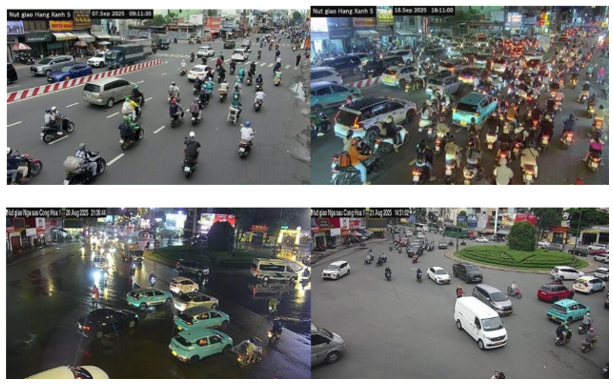
\includegraphics[width=\columnwidth]{fig/samples_pictures_get_from_api.png}
\caption{Sample surveillance camera feeds captured from the Ho Chi Minh City Traffic Portal API across diverse urban intersections.}
\label{fig:api_samples}
\end{figure}

\subsubsection{Graph Edges and RBF Adjacency Matrix}
Graph edges $\mathcal{E}$ represent physical road connections between adjacent camera stations. Edge weights $W_{ij} \in [0, 1]$ are derived from topological road travel distances $d_{ij}$ using a Radial Basis Function (RBF) kernel:
\begin{equation}
W_{ij} = \begin{cases} \exp\left(-\frac{d_{ij}^2}{\sigma^2}\right), & \text{if } i \neq j \text{ and } d_{ij} \le \tau \\ 0, & \text{otherwise,} \end{cases}
\end{equation}
where $\sigma$ is the standard deviation of road distances and $\tau$ is the spatial distance cutoff threshold.

The normalized Graph Laplacian $L$ and Scaled Laplacian $\tilde{L}$ are computed as:
\begin{equation}
L = I_N - D^{-1/2} W D^{-1/2}, \quad \tilde{L} = \frac{2}{\lambda_{\max}} L - I_N,
\end{equation}
where $D_{ii} = \sum_{j} W_{ij}$ is the diagonal degree matrix and $\lambda_{\max}$ is the maximum eigenvalue of $L$.

\subsubsection{Historical Feature Tensor and Target Horizon}
Outputs from Sub-problem 1 are aggregated at 5-minute intervals. Each node $i$ contains a 4-dimensional feature vector $\mathbf{x}_{i,t} \in \mathbb{R}^4$:
\begin{enumerate}
    \item Normalized total vehicle volume $v_{i,t}$.
    \item Sine time-of-day feature: $\sin\left(\frac{2\pi \cdot \text{tod}}{1440}\right)$.
    \item Cosine time-of-day feature: $\cos\left(\frac{2\pi \cdot \text{tod}}{1440}\right)$.
    \item Normalized hour of day: $\frac{\text{hour}}{24}$.
\end{enumerate}

Given historical time series over $T_{\text{in}} = 24$ steps (120 minutes of history), the historical input tensor is $X \in \mathbb{R}^{B \times T_{\text{in}} \times N \times F}$ ($F=4$). The target is forecasting future traffic volume across horizon $H = 6$ steps (30 minutes ahead): $Y \in \mathbb{R}^{B \times H \times N \times 1}$.

\subsection{Sub-Problem 2: TA-STGCN Network Architecture}

TA-STGCN couples Chebyshev Spectral Graph Convolutions \cite{chebnet}, 1D Gated Temporal Convolutions (GLU) \cite{stgcn}, and Model-Level Multi-Head Temporal Self-Attention \cite{attention}. Figure~\ref{fig:stgcn_architecture} illustrates the structural diagram of the TA-STGCN architecture.

\begin{figure}[htbp]
\centering
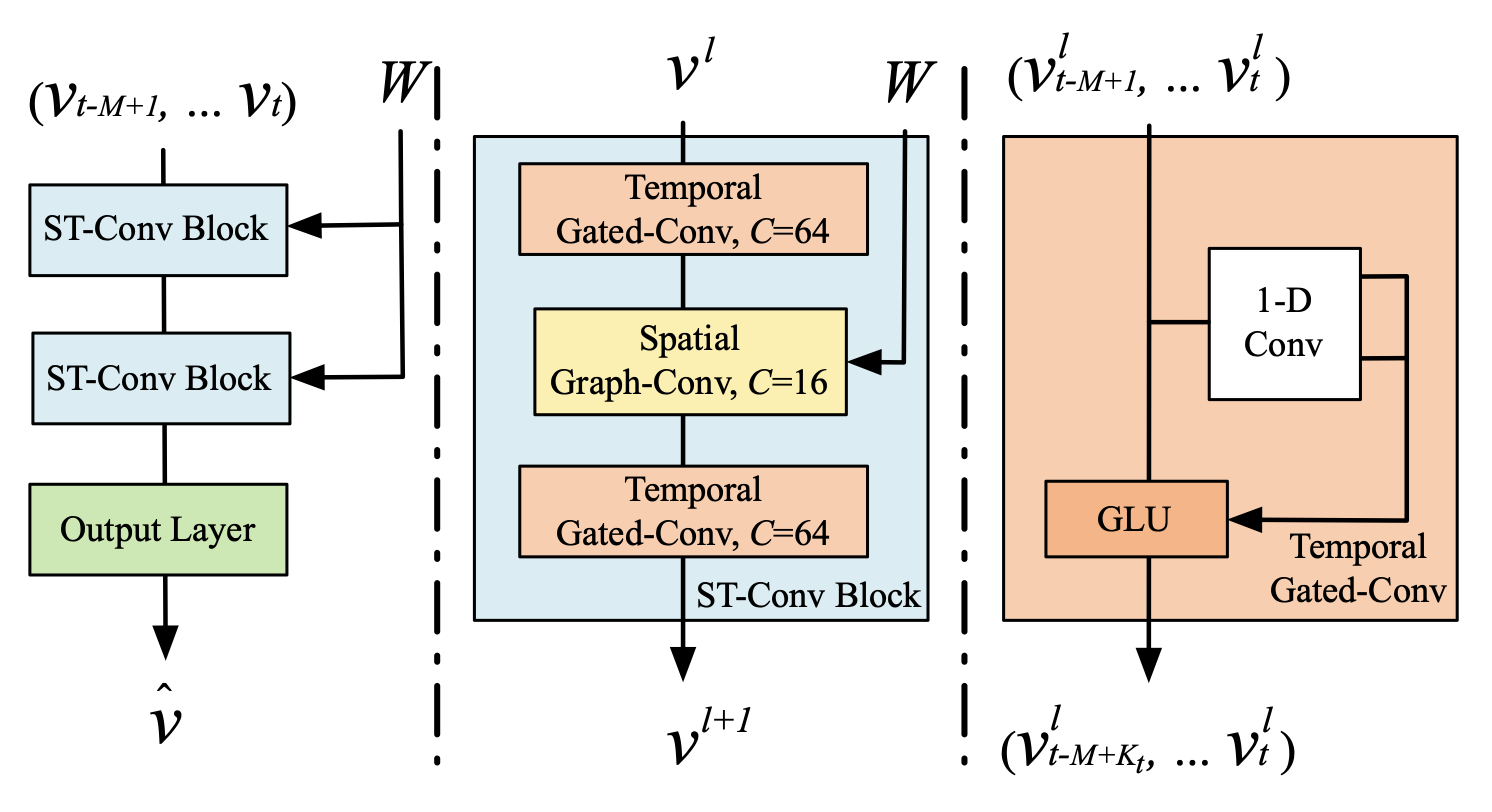
\includegraphics[width=\columnwidth]{fig/stgcn_architecture.png}
\caption{Architectural overview of TA-STGCN, integrating Chebyshev Spectral Graph Convolutions, 1D Temporal GLU blocks, and Model-Level Multi-Head Temporal Self-Attention.}
\label{fig:stgcn_architecture}
\end{figure}

\subsubsection{1D Temporal Gated Convolution (GLU)}
For feature map $H \in \mathbb{R}^{B \times C_{\text{in}} \times N \times T}$, 1D causal convolution doubles channels to $2 C_{\text{out}}$ \cite{stgcn}:
\begin{equation}
\text{Conv}_{1D}(H) = [P, Q] \in \mathbb{R}^{B \times 2 C_{\text{out}} \times N \times T'},
\end{equation}
\begin{equation}
\text{GLU}(H) = P \odot \sigma(Q) \in \mathbb{R}^{B \times C_{\text{out}} \times N \times T'},
\end{equation}
where $\odot$ denotes element-wise product and $\sigma(\cdot)$ is the sigmoid gate.

\subsubsection{Chebyshev Spectral Graph Convolution (ChebNet)}
Spatial graph convolution is approximated using truncated Chebyshev polynomials up to order $K=3$ \cite{chebnet}:
\begin{equation}
g_{\theta} \star_{\mathcal{G}} x \approx \sum_{k=0}^{K-1} \mathbf{\Theta}_k T_k(\tilde{L}) x,
\end{equation}
where $T_0(\tilde{L}) = I_N$, $T_1(\tilde{L}) = \tilde{L}$, and $T_k(\tilde{L}) = 2 \tilde{L} T_{k-1}(\tilde{L}) - T_{k-2}(\tilde{L})$.

\subsubsection{ST-Conv Block Assembly}
Each $ST\text{-Conv}$ block sandwiches spatial ChebNet graph convolution between two temporal GLUs with residual connection and LayerNorm \cite{stgcn}:
\begin{equation}
H^{(1)} = \text{GLU}_1(X), \quad H^{(2)} = \text{ReLU}\left( \text{ChebConv}\left(H^{(1)}, \tilde{L}\right) \right),
\end{equation}
\begin{equation}
H^{(3)} = \text{GLU}_2\left(H^{(2)}\right),
\end{equation}
\begin{equation}
H_{\text{block}} = \text{Dropout}\left( \text{LayerNorm}\left( H^{(3)} + \text{Residual}(X) \right) \right).
\end{equation}

\subsubsection{Model-Level Multi-Head Temporal Self-Attention}
To capture dynamic long-range temporal dependencies across the 24-step historical window, TA-STGCN applies \textbf{Multi-Head Temporal Self-Attention} \cite{attention} at the model output stage (post ST-Conv blocks).

The feature tensor $H_{\text{stgcn}} \in \mathbb{R}^{B \times C \times N \times T}$ is permuted and reshaped into node sequence batches:
\begin{equation}
Z = \text{Reshape}\left(\text{Permute}(H_{\text{stgcn}})\right) \in \mathbb{R}^{(B \cdot N) \times T \times C}.
\end{equation}

For $h=4$ attention heads \cite{attention}, Query, Key, and Value matrices are projected:
\begin{equation}
Q_m = Z W_m^Q, \quad K_m = Z W_m^K, \quad V_m = Z W_m^V, \quad m \in \{1, \dots, h\}.
\end{equation}
Scaled dot-product attention per head is computed as:
\begin{equation}
\text{head}_m = \text{Softmax}\left( \frac{Q_m K_m^T}{\sqrt{d_k}} \right) V_m, \quad d_k = C / h.
\end{equation}
\begin{equation}
\text{MHA}(Z) = \text{Concat}(\text{head}_1, \dots, \text{head}_h) W^O.
\end{equation}

A Transformer-style block \cite{attention} with residual connection, LayerNorm, and GELU Feed-Forward Network (FFN) updates temporal representations:
\begin{equation}
Z^{(1)} = \text{LayerNorm}\left( Z + \text{MHA}(Z) \right),
\end{equation}
\begin{equation}
Z^{(2)} = \text{LayerNorm}\left( Z^{(1)} + \text{FFN}(Z^{(1)}) \right),
\end{equation}
where $\text{FFN}(u) = \text{Linear}_{2}\left( \text{Dropout}\left( \text{GELU}\left( \text{Linear}_{1}(u) \right) \right) \right)$ with 4x dimension expansion ($C \to 4C \to C$).

\subsubsection{Output Conv1D Time-Reduction \& Objective Function}
The attention output tensor $Z^{(2)}$ is permuted back to $\mathbb{R}^{(B \cdot N) \times C \times T}$ and passed to a 1D output convolution with kernel size $T_{\text{in}}$ to collapse time dimension $T_{\text{in}} \to 1$:
\begin{equation}
\hat{Y} = \text{Reshape}\left( \text{Conv1D}_{T_{\text{in}} \to 1}\left(Z^{(2)}\right) \right) \in \mathbb{R}^{B \times H \times N \times 1}.
\end{equation}

The network is trained end-to-end using Pure Huber Loss \cite{huber} ($\delta = 1.0$):
\begin{equation}
\mathcal{L}_{\text{GNN}}(Y, \hat{Y}) = \begin{cases} \frac{1}{2}(Y - \hat{Y})^2, & \text{if } |Y - \hat{Y}| \le \delta \\ \delta |Y - \hat{Y}| - \frac{1}{2}\delta^2, & \text{otherwise.} \end{cases}
\end{equation}

\section{Representation Learning and Classification Baselines}

\subsection{Feature Backbone, Projection Head, and Classification Baseline}
Sau khi tập test được đóng băng (frozen), bài toán nhận diện và học biểu diễn được phát triển dựa trên cấu trúc backbone và đầu chiếu (projection head) phi tuyến. Đối với downstream tasks sử dụng Metric Learning hoặc Self-Supervised Learning, mạng ConvNeXt-Tiny \cite{convnext} được sử dụng làm feature backbone để trích xuất đặc trưng $u_i$. Đặc trưng này đi qua một projection head gồm hai tầng fully-connected với hàm kích hoạt ReLU để sinh embedding chuẩn hóa $L_2$ ký hiệu là $v_i\in\mathbb{R}^{256}$:
\begin{equation}
\tilde{v}_i=W_2\,\mathrm{ReLU}(W_1u_i+b_1)+b_2,\qquad
v_i=\frac{\tilde{v}_i}{\|\tilde{v}_i\|_2}.
\label{eq:projection_head}
\end{equation}

Để thiết lập hệ quy chiếu so sánh, chúng tôi xây dựng mô hình Image Classification Baseline sử dụng ConvNeXt-Tiny làm backbone kết hợp với classifier head (gồm một lớp fully-connected trực tiếp) dự đoán trực tiếp xác suất phân loại của 19 loài gỗ. Nhằm giải quyết vấn đề class imbalance (mất cân bằng dữ liệu lớp) trong bộ dữ liệu, mô hình baseline được huấn luyện bằng hàm Focal Loss thay vì Cross Entropy thông thường. Công thức Focal Loss cho một batch kích thước $B$ được định nghĩa:
\begin{equation}
L_{\text{Focal}} = -\frac{1}{B} \sum_{i=1}^{B} \alpha (1 - p_{t, i})^\gamma \log(p_{t, i})
\label{eq:focal_loss}
\end{equation}
trong đó $p_{t, i}$ là xác suất dự đoán của mô hình đối với lớp đúng của mẫu $i$, $\gamma$ là focusing parameter giúp mô hình tập trung vào các mẫu khó phân loại, và $\alpha$ là hệ số cân bằng. Trong thực nghiệm, các tham số này được thiết lập lần lượt là $\gamma = 2.0$ và $\alpha = 0.25$. Mạng ConvNeXt-Tiny được freeze $90\%$ số lượng lớp để hạn chế overfitting trên tập dữ liệu gỗ có số lượng mẫu hạn chế. Bộ tối ưu hóa AdamW với learning rate khởi tạo $5\times 10^{-4}$ và weight decay $10^{-2}$ kết hợp với Cosine Annealing learning rate scheduler được sử dụng trong suốt quá trình training. Mọi thuật toán metric learning hoặc self-supervised learning thay thế loss function nhưng không thay đổi manifest, split, augmentation cơ sở hoặc quy tắc lựa chọn trên validation. Nhờ đó, khác biệt quan sát được giữa các phương pháp nhận diện không bị lẫn với khác biệt do split dữ liệu.

\subsection{Deep Metric Learning Loss Functions and Baselines}
Để đánh giá khách quan các hướng học biểu diễn đặc trưng, chúng tôi thực nghiệm đối chiếu 14 hàm loss học khoảng cách trong cùng một quy trình huấn luyện thống nhất về mạng cơ sở, bộ đầu chiếu, tăng cường dữ liệu và giao thức CEGS-Split. Ký hiệu chung: $\mathbf{z}_i\in\mathbb{R}^{D}$ là đặc trưng nhúng đã chuẩn hóa $L_2$, $y_i$ là nhãn loài, $d_{ij}=\|\mathbf{z}_i-\mathbf{z}_j\|_2$ là khoảng cách Euclid, $S_{ij}=\mathbf{z}_i^T\mathbf{z}_j$ là cosine similarity và $[u]_+=\max(0,u)$.

\subsubsection{Standard Triplet Loss}
Triplet Loss tối ưu hóa mối quan hệ giữa bộ ba mẫu gồm mẫu neo (anchor) $a$, mẫu tích cực (positive) $p$ thuộc cùng loài và mẫu tiêu cực (negative) $n$ thuộc loài khác. Mục tiêu của hàm loss là thu hẹp khoảng cách giữa mẫu neo và mẫu tích cực, đồng thời đẩy mẫu tiêu cực ra xa hơn mẫu neo ít nhất một khoảng biên (margin) $\alpha$:
\begin{equation}
L_{\text{triplet}}=\frac{1}{|\mathcal{T}|}\sum_{(a,p,n)\in\mathcal{T}}\left[d(a,p)^2-d(a,n)^2+\alpha\right]_+.
\end{equation}

\subsubsection{Semi-hard Triplet Loss}
Phương pháp Triplet bán khó (Semi-hard Triplet Loss) lựa chọn các mẫu tiêu cực (negative) không quá dễ nhưng cũng không quá nhiễu. Với một cặp mẫu neo và mẫu tích cực $(a,p)$, mẫu tiêu cực $n$ được chọn nếu thỏa mãn:
\begin{equation}
d(a,p)^2<d(a,n)^2<d(a,p)^2+\alpha.
\end{equation}
Loss vẫn giữ dạng triplet chuẩn:
\begin{equation}
L_{\text{semi-hard}}=\frac{1}{|\mathcal{T}_{sh}|}\sum_{(a,p,n)\in\mathcal{T}_{sh}}\left[d(a,p)^2-d(a,n)^2+\alpha\right]_+.
\end{equation}

\subsubsection{Soft-Margin Triplet Loss}
Phương pháp Triplet biên mềm (Soft-Margin Triplet) thay thế hàm hinge cứng bằng hàm log-sum-exp mịn:
\begin{equation}
L_{\text{soft-triplet}}=\frac{1}{N}\sum_{i=1}^{N}\log\left[1+e^{d(a_i,p_i)^2-d(a_i,n_i)^2}\right].
\end{equation}

\subsubsection{Angular Loss}
Hàm loss Angular (Angular Loss) tối ưu hóa quan hệ góc của tam giác được tạo bởi bộ ba mẫu (triplet) thay vì chỉ tối ưu hóa khoảng cách Euclid đơn thuần:
\begin{equation}
L_{\text{angular}}=\frac{1}{|\mathcal{T}|}\sum_{(a,p,n)\in\mathcal{T}}\log\left[1+e^{\Delta_{\theta}(a,p,n)}\right],
\end{equation}
Trong đó:
\begin{equation}
\begin{aligned}
\Delta_{\theta}(a,p,n) = &4\tan^2\alpha(\mathbf{z}_a+\mathbf{z}_p)^T\mathbf{z}_n \\
&- 2(1+\tan^2\alpha)\mathbf{z}_a^T\mathbf{z}_p.
\end{aligned}
\end{equation}

\subsubsection{Multi-Similarity Loss}
Multi-Similarity Loss khai thác đồng thời thông tin từ nhiều cặp tích cực và tiêu cực trong cùng một lô dữ liệu, đồng thời gán trọng số lớn hơn cho các cặp có độ khó cao:
\begin{equation}
L_{\text{MS}}=\frac{1}{N}\sum_{i=1}^{N} \left[ \phi^+(P_i) + \phi^-(N_i) \right],
\end{equation}
Trong đó:
\begin{equation}
\begin{aligned}
\phi^+(P_i) &= \frac{1}{\alpha}\log\left[1+\sum_{p\in P_i}e^{-\alpha(S_{ip}-\lambda)}\right], \\
\phi^-(N_i) &= \frac{1}{\beta}\log\left[1+\sum_{n\in N_i}e^{\beta(S_{in}-\lambda)}\right].
\end{aligned}
\end{equation}

\subsubsection{Standard Contrastive Loss}
Contrastive Loss tối ưu hóa khoảng cách trên từng cặp mẫu riêng lẻ:
\begin{equation}
L_{\text{contrastive}}=(1-q_{ij})\frac{1}{2}d_{ij}^{2}+q_{ij}\frac{1}{2}[m-d_{ij}]_+^2.
\end{equation}

\subsubsection{Online Hard Contrastive Loss}
Phương pháp tương phản khai thác mẫu khó trực tuyến (Online Hard Contrastive) tập trung tối ưu hóa trên cặp tích cực xa nhất và cặp tiêu cực gần nhất trong cùng một lô dữ liệu (batch):
\begin{equation}
d_{\text{pos\_max}}^i=\max_{p:y_p=y_i,p\ne i}d_{ip},\quad d_{\text{neg\_min}}^i=\min_{n:y_n\ne y_i}d_{in}.
\end{equation}
\begin{equation}
L_{\text{hard-cont}}=\frac{1}{B}\sum_{i=1}^{B}\left[(d_{\text{pos\_max}}^i)^2+[m-d_{\text{neg\_min}}^i]_+^2\right].
\end{equation}

\subsubsection{Lifted Structured Loss}
Lifted Structured Loss mở rộng cơ chế học tương phản bằng cách đồng thời xem xét tất cả các mẫu tiêu cực liên quan đến một cặp mẫu tích cực $(i,j)$:
\begin{equation}
L_{\text{lifted}}=\frac{1}{2|P|}\sum_{(i,j)\in P}\left[d_{ij}+\log\left(\Phi(i, j)\right)\right]_+^2,
\end{equation}
Trong đó:
\begin{equation}
\begin{aligned}
\Phi(i, j) = &\sum_{k:y_k\ne y_i}e^{\alpha-d_{ik}} \\
&+ \sum_{k:y_k\ne y_j}e^{\alpha-d_{jk}}.
\end{aligned}
\end{equation}

\subsubsection{Circle Loss}
Circle Loss đề xuất một cách tiếp cận tối ưu hóa độ tương đồng thống nhất, trong đó các mẫu tích cực và tiêu cực được gán các trọng số tự điều chỉnh:
\begin{equation}
L_{\text{circle}} = \log \left[ 1 + \Omega_{\text{circle}}(i) \right],
\end{equation}
Trong đó:
\begin{equation}
\begin{aligned}
\Omega_{\text{circle}}(i) = &\sum_{n\in N_i}e^{\gamma\alpha_n(S_{in}-\Delta_n)} \times \\
&\sum_{p\in P_i}e^{-\gamma\alpha_p(S_{ip}-\Delta_p)},
\end{aligned}
\end{equation}
and:
\begin{equation}
\alpha_p=[O_p-S_{ip}]_+, \quad \alpha_n=[S_{in}-O_n]_+.
\end{equation}

\subsubsection{Proxy Anchor Loss}
Phương pháp Proxy Anchor thay thế việc so sánh trực tiếp giữa các hình ảnh bằng việc so sánh hình ảnh với các mẫu đại diện (proxy) của từng lớp:
\begin{equation}
L_{\text{PA}} = \frac{1}{|P^+|}\sum_{p\in P^+}\log \Gamma^+(p) + \frac{1}{|P|}\sum_{p\in P}\log \Gamma^-(p),
\end{equation}
Trong đó:
\begin{equation}
\begin{aligned}
\Gamma^+(p) &= 1+\sum_{\mathbf{z}\in X_p^+}e^{-\alpha(S(\mathbf{z},p)-\delta)}, \\
\Gamma^-(p) &= 1+\sum_{\mathbf{z}\in X_p^-}e^{\alpha(S(\mathbf{z},p)+\delta)}.
\end{aligned}
\end{equation}

\subsubsection{ArcFace Loss}
Phương pháp ArcFace (Additive Angular Margin Loss) áp dụng trực tiếp một biên góc cộng (additive angular margin) vào giá trị logit của lớp chính xác:
\begin{equation}
\begin{aligned}
L_{\text{ArcFace}} = -\frac{1}{N}\sum_{i=1}^{N}\log \frac{e^{s\cos(\theta_{y_i}+m)}}{\Lambda_i},
\end{aligned}
\end{equation}
Trong đó:
\begin{equation}
\begin{aligned}
\Lambda_i = e^{s\cos(\theta_{y_i}+m)} + \sum_{j\ne y_i}e^{s\cos\theta_j}.
\end{aligned}
\end{equation}

\subsubsection{SubCenter ArcFace Loss}
Phương pháp SubCenter ArcFace mở rộng thuật toán ArcFace bằng cách gán nhiều trọng tâm phụ (sub-center) cho mỗi lớp. Với cấu hình $K$ trọng tâm phụ cho mỗi loài, giá trị logit của lớp chính xác được tính toán dựa trên trọng tâm phụ gần nhất:
\begin{equation}
\cos\theta_{y_i}=\max_{k=1}^{K}\frac{\mathbf{z}_i^T W_{y_i}^{(k)}}{\|\mathbf{z}_i\|_2\|W_{y_i}^{(k)}\|_2}.
\end{equation}

\subsubsection{SoftTriple Loss}
Tương tự, phương pháp SoftTriple cũng sử dụng nhiều trọng tâm đại diện cho mỗi lớp nhưng áp dụng cơ chế gán mềm (soft assignment) thay vì lấy giá trị cực đại:
\begin{equation}
S_{i,c}=\sum_{k=1}^{K}\frac{e^{\mathbf{z}_i^T w_c^{(k)}/\gamma}}{\sum_{t=1}^{K}e^{\mathbf{z}_i^T w_c^{(t)}/\gamma}}\mathbf{z}_i^T w_c^{(k)}.
\end{equation}
Loss phân loại có margin:
\begin{equation}
L_{\text{SoftTriple}}=-\log\frac{e^{\lambda(S_{i,y_i}-\delta)}}{e^{\lambda(S_{i,y_i}-\delta)}+\sum_{c\ne y_i}e^{\lambda S_{i,c}}}.
\end{equation}

\subsubsection{Supervised Contrastive Loss (SupCon)}
Contrastive Loss có giám sát (Supervised Contrastive Loss - SupCon) mở rộng phương pháp SimCLR sang học có giám sát bằng cách coi tất cả các mẫu thuộc cùng một loài trong lô dữ liệu là các mẫu tích cực của nhau:
\begin{equation}
L_{\text{SupCon}}=\sum_{i\in I}\frac{-1}{|P(i)|}\sum_{p\in P(i)}\log\frac{e^{\mathbf{z}_i^T\mathbf{z}_p/\tau}}{\sum_{a\in A(i)}e^{\mathbf{z}_i^T\mathbf{z}_a/\tau}}.
\end{equation}
SupCon tối ưu hóa việc sắp đặt đặc trưng trên toàn bộ lô dữ liệu và thường tạo ra không gian nhúng có khả năng chuyển giao tốt.

\subsection{Self-Supervised Learning Loss Functions}
Trong học biểu diễn tự giám sát (Self-Supervised Learning - SSL), mô hình thực hiện tối ưu hóa đặc trưng thông qua các biến thể tăng cường ngẫu nhiên của hình ảnh mà không cần sử dụng nhãn lớp giám sát. Phần này trình bày các hàm loss của bốn phương pháp học tự giám sát được khảo sát trong nghiên cứu.

\subsubsection{SimCLR Loss}
Phương pháp SimCLR (Simple Framework for Contrastive Learning of Visual Representations) tối ưu hóa hàm loss tương phản InfoNCE trên các cặp ảnh tăng cường. Với kích thước lô dữ liệu là $N$, mỗi hình ảnh được tăng cường ngẫu nhiên thành 2 phiên bản (views), tạo thành một lô gồm $2N$ mẫu dữ liệu. Cặp mẫu tích cực (positive pair) là $(i,j)$ gồm hai phiên bản tăng cường khác nhau của cùng một hình ảnh gốc. Hàm loss cho mỗi cặp mẫu tích cực $(i,j)$ được phát biểu:
\begin{equation}
\begin{aligned}
\ell(i, j) = -\log \frac{e^{\mathbf{z}_i^T\mathbf{z}_j/\tau}}{\Omega_i},
\end{aligned}
\end{equation}
Trong đó:
\begin{equation}
\begin{aligned}
\Omega_i = \sum_{k=1}^{2N} \mathbb{I}_{[k \ne i]} e^{\mathbf{z}_i^T\mathbf{z}_k/\tau}.
\end{aligned}
\end{equation}
trong đó $\tau$ là siêu tham số nhiệt độ (temperature). Hàm loss tổng thể được tính bằng macro average của toàn bộ các cặp mẫu tích cực trong lô dữ liệu:
\begin{equation}
L_{\text{SimCLR}} = \frac{1}{2N} \sum_{k=1}^{N} \left[ \ell(2k-1, 2k) + \ell(2k, 2k-1) \right].
\end{equation}

\subsubsection{BYOL Loss}
Phương pháp BYOL (Bootstrap Your Own Latent) sử dụng hai mạng nơ-ron song song: mạng học trực tiếp (online network) với tham số $\theta$ và target network với tham số $\xi$. Mạng học trực tiếp có nhiệm vụ dự đoán biểu diễn của mạng mục tiêu từ một phiên bản ảnh khác. BYOL tối ưu hóa sai số bình phương trung bình (MSE) giữa vector dự đoán đã chuẩn hóa của mạng trực tiếp và vector đặc trưng của mạng mục tiêu:
\begin{equation}
L_{\text{MSE}}(q_\theta(z_\theta), z'_\xi) = \left\| \bar{q}_\theta - \bar{z}'_\xi \right\|_2^2 = 2 - 2 \bar{q}_\theta^T \bar{z}'_\xi,
\end{equation}
Trong đó:
\begin{equation}
\bar{q}_\theta = \frac{q_\theta(z_\theta)}{\|q_\theta(z_\theta)\|_2},\quad \bar{z}'_\xi = \frac{z'_\xi}{\|z'_\xi\|_2}.
\end{equation}
Việc ngăn chặn hiện tượng sụp đổ biểu diễn đặc trưng (representation collapse) được đảm bảo bằng cơ chế dừng cập nhật đạo hàm (\textit{stop-gradient}) đặt trên mạng mục tiêu:
\begin{equation}
L_{\text{BYOL}} = L_{\text{MSE}}(q_\theta(z_\theta), \text{stop\_gradient}(z'_\xi)).
\end{equation}
Tham số mạng mục tiêu $\xi$ được cập nhật chậm theo cơ chế trung bình trượt lũy thừa (EMA) từ $\theta$:
\begin{equation}
\xi \leftarrow m \xi + (1-m) \theta,
\end{equation}
trong đó $m \in [0, 1]$ là hệ số momentum.

\subsubsection{SimSiam Loss}
Phương pháp SimSiam (Simple Siamese) đơn giản hóa kiến trúc BYOL bằng cách loại bỏ hoàn toàn momentum target network (momentum target network, tức thiết lập $\xi = \theta$). SimSiam chứng minh rằng chỉ cần sử dụng cơ chế dừng cập nhật đạo hàm kết hợp với kiến trúc không đối xứng (bộ dự đoán predictor) là đủ để ngăn chặn sự sụp đổ biểu diễn đặc trưng. Hàm loss đối xứng được định nghĩa như sau:
\begin{equation}
L_{\text{SimSiam}} = \frac{1}{2} \mathcal{D}\big(p_1, \text{sg}(z_2)\big) + \frac{1}{2} \mathcal{D}\big(p_2, \text{sg}(z_1)\big),
\end{equation}
trong đó $p_1 = q_\theta(z_1)$ và $p_2 = q_\theta(z_2)$ là đầu ra của bộ dự đoán cho hai phiên bản ảnh, còn $z_1, z_2$ là đầu ra của bộ đầu chiếu. $\text{sg}$ biểu thị toán tử dừng đạo hàm (stop-gradient). $\mathcal{D}$ là cosine similarity âm:
\begin{equation}
\mathcal{D}(p, z) = -\frac{p^T z}{\|p\|_2 \|z\|_2}.
\end{equation}

\subsubsection{Barlow Twins Loss}
Phương pháp Barlow Twins áp dụng nguyên lý giảm thiểu thông tin dư thừa (redundancy reduction) lên ma trận tương quan chéo thu được từ hai phiên bản ảnh tăng cường. Gọi $C$ là ma trận tương quan chéo kích thước $D \times D$ tính toán dọc theo chiều lô dữ liệu $B$ giữa hai tập đặc trưng chiếu $\mathbf{z}^A$ và $\mathbf{z}^B$:
\begin{equation}
C_{ij} = \frac{\sum_{b=1}^{B} z_{b,i}^A z_{b,j}^B}{\sqrt{\sum_{b=1}^{B} (z_{b,i}^A)^2} \sqrt{\sum_{b=1}^{B} (z_{b,j}^B)^2}},
\end{equation}
trong đó $i, j$ đại diện cho các chiều của không gian đặc trưng nhúng. Hàm mất mát Barlow Twins được định nghĩa là:
\begin{equation}
L_{\text{BarlowTwins}} = \sum_{i=1}^{D} (1 - C_{ii})^2 + \lambda \sum_{i=1}^{D} \sum_{j \neq i} C_{ij}^2,
\end{equation}
trong đó số hạng thứ nhất (invariance term) ép các hệ số tương quan chéo trên đường chéo chính tiến về 1 (tối đa hóa độ tương đồng giữa hai phiên bản ảnh), số hạng thứ hai (redundancy reduction term) ép các hệ số tương quan chéo ngoài đường chéo chính tiến về 0 với hệ số phạt $\lambda > 0$ (giảm thiểu sự trùng lặp thông tin giữa các chiều đặc trưng nhúng).

\section{Experimental Setup}

\subsection{Datasets and Data Preprocessing}

\subsubsection{Sub-Problem 1 Vision Dataset}
The camera vehicle estimation dataset consists of \textbf{6,000 manually annotated traffic images} captured across surveillance cameras from the Ho Chi Minh City Traffic Portal. The dataset is partitioned into:
\begin{itemize}
    \item \textbf{Training Set:} 4,000 images.
    \item \textbf{Validation Set:} 1,000 images.
    \item \textbf{Testing Set:} 1,000 images.
\end{itemize}
Ground-truth annotations provide individual continuous counts for passenger cars and motorbikes. Images are resized to $224 \times 224$ pixels and normalized with ImageNet mean and standard deviation.

\subsubsection{Sub-Problem 2 Traffic Graph Time Series Dataset}
Using Stage 1 predictions across 608 active camera nodes, time series are aggregated at 5-minute intervals ($step\_minutes=5$). Missing steps ($\le 30$ minutes) are linearly interpolated and smoothed via double-rolling transformation ($window_1=3$, $window_2=5$).

Historical lookback length is $T_{\text{in}} = 24$ steps (120 minutes history), and forecast horizon is $H = 6$ steps (30 minutes ahead).

The time-series dataset is split chronologically:
\begin{itemize}
    \item \textbf{Training Set:} First 80\% of the time range.
    \item \textbf{Validation Set:} Middle 10\% of the time range.
    \item \textbf{Testing Set:} Final 10\% of the time range.
\end{itemize}

\subsection{Hyperparameter Settings and Training Details}

All models across both sub-problems are implemented in PyTorch 2.x and trained hardware-accelerated on an **NVIDIA T4 GPU (16 GB VRAM)**.

\subsubsection{Sub-Problem 1 Training Hyperparameters}
The vision backbones (ConvNeXt-Tiny \cite{convnext} and ResNet-50 \cite{resnet}) with custom MLP regression heads are trained under the following setup:
\begin{itemize}
    \item \textbf{Hardware Accelerator:} NVIDIA T4 GPU (16 GB VRAM).
    \item \textbf{Optimizer:} AdamW optimizer with initial learning rate $\eta = 1 \times 10^{-4}$ and weight decay coefficient $1 \times 10^{-2}$.
    \item \textbf{Learning Rate Schedule:} Cosine Annealing Learning Rate Scheduler decaying down to $\eta_{\min} = 1 \times 10^{-6}$.
    \item \textbf{Epochs and Batch Size:} Models are trained for 100 epochs with a mini-batch size of $B = 32$.
    \item \textbf{Loss Function:} Smooth $L_1$ (Huber) Loss \cite{huber} with threshold $\beta = 1.0$.
    \item \textbf{Data Augmentations:} Random horizontal flips (probability $p=0.5$), color jittering ($\pm 15\%$ brightness, contrast, and saturation), and random spatial cropping resized to $224 \times 224$.
\end{itemize}

\subsubsection{Sub-Problem 2 Training Hyperparameters}
The spatio-temporal graph models (GCN-LSTM \cite{gcn, tgcn}, STGCN Baseline \cite{stgcn}, and TA-STGCN \cite{attention}) are trained under the following setup:
\begin{itemize}
    \item \textbf{Hardware Accelerator:} NVIDIA T4 GPU (16 GB VRAM).
    \item \textbf{Optimizer:} Adam optimizer \cite{adam} with initial learning rate $\eta = 5 \times 10^{-4}$ and weight decay coefficient $1 \times 10^{-4}$.
    \item \textbf{Learning Rate Schedule:} ReduceLROnPlateau scheduler decaying the learning rate by a factor of $0.5$ if validation loss fails to improve for 10 consecutive epochs ($\text{patience}=10$).
    \item \textbf{Max Epochs and Early Stopping:} Trained for up to 500 epochs with an early stopping patience of 30 epochs based on Validation MAE.
    \item \textbf{Batch Size:} Training mini-batch size $B = 16$ (evaluation batch size $\min(B, 32) = 16$).
    \item \textbf{Loss Function:} Pure Huber Loss \cite{huber} ($\delta = 1.0$) trained end-to-end.
    \item \textbf{Multi-Seed Evaluation Protocol:} Models are evaluated across \textbf{5 independent random seeds}: $\mathcal{S} = \{42, 100, 2024, 777, 999\}$. All reported metrics present $\text{Mean} \pm \text{Std}$ over the 5 seeds.
\end{itemize}

\subsection{Evaluation Metrics}

Model performance is evaluated using Mean Absolute Error (MAE), Root Mean Squared Error (RMSE), and Mean Squared Error (MSE):
\begin{equation}
\text{MAE} = \frac{1}{N \cdot H \cdot M} \sum_{i=1}^{N} \sum_{h=1}^{H} \sum_{k=1}^{M} \left| y_{i,h}^{(k)} - \hat{y}_{i,h}^{(k)} \right|,
\end{equation}
\begin{equation}
\text{RMSE} = \sqrt{ \frac{1}{N \cdot H \cdot M} \sum_{i=1}^{N} \sum_{h=1}^{H} \sum_{k=1}^{M} \left( y_{i,h}^{(k)} - \hat{y}_{i,h}^{(k)} \right)^2 },
\end{equation}
\begin{equation}
\text{MSE} = \frac{1}{N \cdot H \cdot M} \sum_{i=1}^{N} \sum_{h=1}^{H} \sum_{k=1}^{M} \left( y_{i,h}^{(k)} - \hat{y}_{i,h}^{(k)} \right)^2,
\end{equation}
where $N=608$ graph nodes, $H=6$ forecast steps, and $M$ is the test batch count.

\section{Results and Discussion}

\subsection{Recognition Performance on Held-Out Specimens}
Bảng \ref{tab:baseline_report} báo cáo mô hình baseline ConvNeXt-Tiny dùng Focal Loss trên tập test của CEGS-Split. Accuracy đạt $80.28\%$, macro-F1 đạt $76.77\%$ và weighted-F1 đạt $80.15\%$. Chênh lệch giữa macro-F1 và weighted-F1 cho thấy hiệu năng không đồng đều giữa các loài.

\begin{table}[htbp]
\centering
\caption{Per-species classification report of the baseline model on the CEGS-Split test set.}
\label{tab:baseline_report}
\resizebox{\columnwidth}{!}{%
\begin{tabular}{lcccc}
\toprule
\textbf{Species} & \textbf{Precision} & \textbf{Recall} & \textbf{F1} & \textbf{Support} \\
\midrule
\textit{Afzelia africana} & 0.5833 & 0.5185 & 0.5490 & 54 \\
\textit{Afzelia bella} & 0.0270 & 0.0250 & 0.0260 & 40 \\
\textit{Afzelia pachyloba} & 0.2500 & 0.2955 & 0.2708 & 44 \\
\textit{Afzelia quanzensis} & 0.6628 & 1.0000 & 0.7972 & 57 \\
\textit{Dalbergia cochinchinensis} & 0.9028 & 0.9286 & 0.9155 & 70 \\
\textit{Dalbergia melanoxylon} & 1.0000 & 0.9636 & 0.9815 & 55 \\
\textit{Dalbergia oliveri} & 0.9118 & 1.0000 & 0.9538 & 62 \\
\textit{Dalbergia rimosa} & 0.8571 & 1.0000 & 0.9231 & 30 \\
\textit{Dalbergia tonkinensis} & 0.9565 & 0.7333 & 0.8302 & 30 \\
\textit{Guibourtia arnoldiana} & 1.0000 & 0.5588 & 0.7170 & 34 \\
\textit{Guibourtia coleosperma} & 1.0000 & 0.9861 & 0.9930 & 72 \\
\textit{Guibourtia ehie} & 0.4906 & 0.6500 & 0.5591 & 40 \\
\textit{Peltogyne pubescens} & 1.0000 & 1.0000 & 1.0000 & 110 \\
\textit{Pterocarpus erinaceus} & 0.7882 & 1.0000 & 0.8816 & 67 \\
\textit{Pterocarpus indicus} & 1.0000 & 0.6034 & 0.7527 & 58 \\
\textit{Pterocarpus macrocarpus} & 1.0000 & 0.6667 & 0.8000 & 51 \\
\textit{Pterocarpus soyauxii} & 0.8209 & 1.0000 & 0.9016 & 55 \\
\textit{Sindora cochinchinensis} & 0.9474 & 0.7129 & 0.8136 & 101 \\
\textit{Sindora tonkinensis} & 0.8537 & 1.0000 & 0.9211 & 35 \\
\midrule
\textbf{Accuracy} & \multicolumn{2}{c}{---} & 0.8028 & 1065 \\
\textbf{Macro avg.} & 0.7922 & 0.7707 & 0.7677 & 1065 \\
\textbf{Weighted avg.} & 0.8250 & 0.8028 & 0.8015 & 1065 \\
\bottomrule
\end{tabular}%
}
\end{table}

Các loài \textit{A. bella} và \textit{A. pachyloba} thuộc chi \textit{Afzelia} là những lớp khó nhất trong phép thử này. Kết quả này phù hợp với nhận định rằng bài toán còn chứa biến thiên nội loài và ranh giới hình thái hẹp; nó không cho phép quy kết nguyên nhân chỉ từ một ma trận nhầm lẫn. Hình \ref{fig:confusion_matrix} cung cấp chi tiết các cặp nhầm lẫn để định hướng kiểm tra ảnh gốc, nhãn và quy trình thu nhận.

\begin{figure}[htbp]
\centering
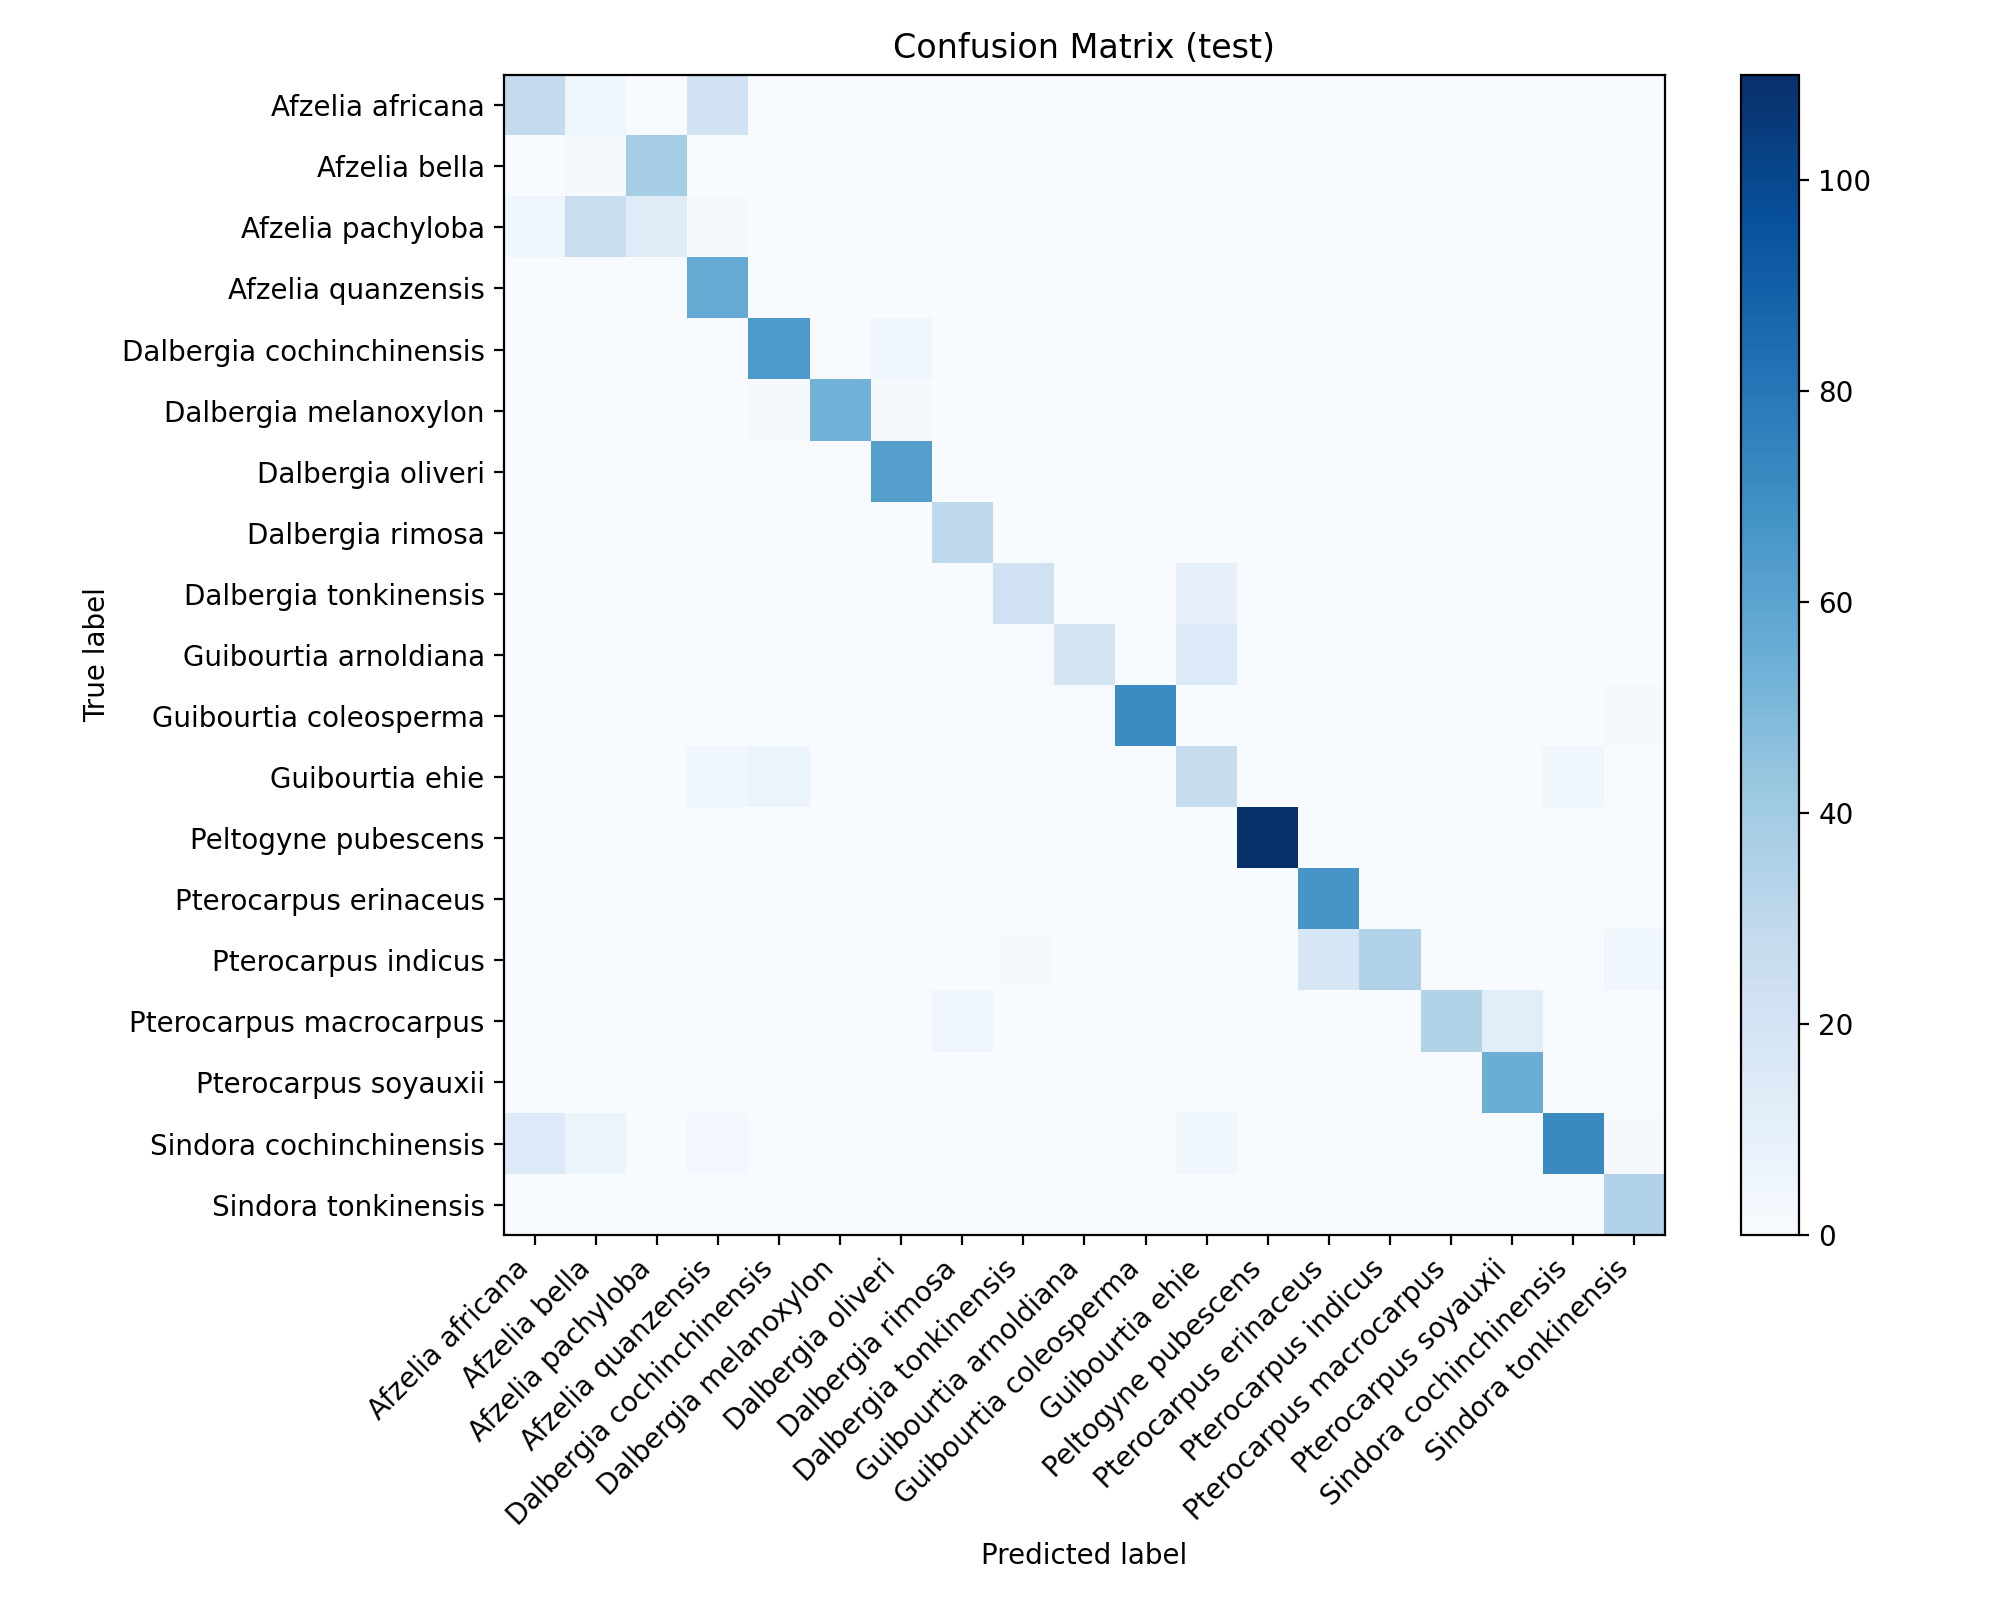
\includegraphics[width=\columnwidth]{fig/confusion_matrix_test.png}
\caption{Confusion matrix of the baseline model on the CEGS-Split test set.}
\label{fig:confusion_matrix}
\end{figure}

\subsection{Sensitivity to the Split Unit}
Bảng \ref{tab:split_ablation} so sánh KNN trên embedding Swin-Large đóng băng (frozen Swin-Large) giữa random image split và CEGS-Split. Random image split đạt KNN accuracy trung bình $0.9581$, trong khi CEGS-Split đạt $0.9087$; chênh lệch là $0.0494$ điểm tuyệt đối. Macro-F1 thay đổi từ $0.9493$ xuống $0.8858$. Vì feature extractor và bộ phân loại KNN được giữ nguyên, thí nghiệm cho thấy đơn vị split có thể thay đổi đáng kể kết quả evaluation.

\begin{table*}[htbp]
\centering
\caption{Sensitivity of KNN on frozen Swin-Large embeddings to the data split. Cosine similarity is reported as an inter-split image-level statistic.}
\label{tab:split_ablation}
\resizebox{\textwidth}{!}{%
\begin{tabular}{llccccccc}
\toprule
\textbf{Split} & \textbf{Seed} & \textbf{KNN Acc.} & \textbf{Macro-F1} & \textbf{Weighted-F1} & \textbf{Mean CosSim} & \textbf{Max CosSim} & \textbf{Train} & \textbf{Test} \\
\midrule
Random image & 42 & 0.9522 & 0.9343 & 0.9495 & 0.5678 & 0.9139 & 3900 & 1026 \\
Random image & 123 & 0.9429 & 0.9390 & 0.9426 & 0.5754 & 0.9173 & 3963 & 1015 \\
Random image & 456 & 0.9793 & 0.9745 & 0.9792 & 0.5758 & 0.9171 & 3895 & 1064 \\
CEGS-Split & 42 & 0.9087 & 0.8858 & 0.9062 & 0.5711 & 0.8999 & 4151 & 1041 \\
\midrule
Random image (mean) & --- & $0.9581 \pm 0.0155$ & $0.9493 \pm 0.0179$ & $0.9571 \pm 0.0159$ & $0.5730 \pm 0.0037$ & $0.9161 \pm 0.0015$ & --- & --- \\
CEGS-Split & --- & 0.9087 & 0.8858 & 0.9062 & 0.5711 & 0.8999 & --- & --- \\
\bottomrule
\end{tabular}%
}
\end{table*}

Độ tương đồng cosine cực đại (max cosine similarity) giảm từ $0.9161$ xuống $0.8999$ khi dùng CEGS-Split, còn mean cosine similarity thay đổi nhỏ. Đây là dấu hiệu nhất quán với việc random image split tạo ra một số cặp train--test gần nhau hơn; tuy nhiên các số cosine không tự chứng minh rằng một cặp ảnh có cùng nguồn. Kết luận về rò rỉ phải dựa trên giao của \texttt{specimen\_id} giữa các tập và kiểm tra manifest. Theo cách diễn giải thận trọng, kết quả trên chỉ xác lập rằng điểm số của cùng một pipeline nhạy với cách nhóm các ảnh thành đơn vị split.

CEGS-Split không được thiết kế để làm bài toán dễ hơn hoặc khó hơn một cách tùy ý. Nó xác định câu hỏi đánh giá khác: nhận diện một ảnh từ mẫu vật chưa xuất hiện trong quá trình training (held-out specimens). Do đó, chênh lệch $4.94$ điểm phần trăm không nên được gọi là mức đánh giá quá cao có thể khái quát cho mọi bộ dữ liệu; đây là mức khác biệt quan sát được trên S3, embedding và cấu hình KNN hiện tại.

\subsection{Implications for Representation Learning Benchmarks}
Kết quả cho thấy benchmark các loss functions chỉ có ý nghĩa khi split được khóa (frozen) trước khi thực hiện. Với cùng CEGS-Split, các phương pháp metric learning và self-supervised learning có thể được so sánh bằng retrieval, clustering và macro-F1. Khi công bố kết quả đầy đủ, mỗi phương pháp cần báo cáo seed, checkpoint selection rule, số specimen trong mỗi tập và độ biến thiên qua các lần chạy. Báo cáo một điểm số duy nhất trên random image split không đủ để tách biệt tác động của kiến trúc mạng khỏi tác động của cấu trúc split dữ liệu.

\subsection{Limitations}
Thứ nhất, kết quả CEGS-Split hiện dựa trên một split đã khóa; vì thế chưa thể suy ra khoảng tin cậy của chính protocol. Thứ hai, khả năng tổng quát hóa ngoài S3, đặc biệt sang thiết bị, điều kiện bề mặt hoặc nguồn mẫu khác, chưa được kiểm chứng bằng external test set. Thứ ba, độ tin cậy của split theo mẫu vật phụ thuộc trực tiếp vào độ đầy đủ của manifest. Những giới hạn này là động cơ để phát hành manifest phiên bản hóa, nhiều group-disjoint split và một tập test ngoài nguồn (external test set) trong các nghiên cứu tiếp theo.

\section{Qualitative Analysis and Visual Interpretability}

\subsection{Visual Attention Verification in Sub-Problem 1}
To verify that Stage 1 ConvNeXt-Tiny vehicle count regression grounds its predictions in physical vehicle visual features rather than background environmental shortcuts (such as road markings, tree shadows, or weather glare), we analyze feature attribution maps using visual attention visualizations.

Figure~\ref{fig:attention_map} presents attention heatmaps generated by the ConvNeXt-Tiny vehicle counting model across representative traffic camera scenes.

\begin{figure}[htbp]
\centering
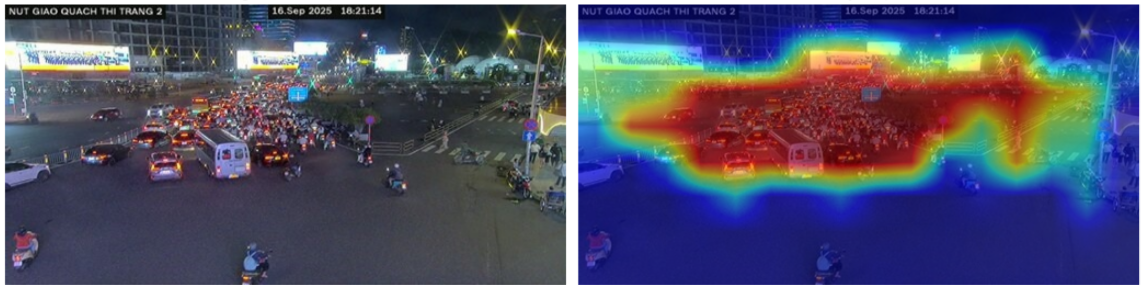
\includegraphics[width=\columnwidth]{fig/attention_map.png}
\caption{Visual attention heatmaps generated by ConvNeXt-Tiny vehicle count regression model, confirming high attention focus on vehicles (motorbikes and cars) in camera feeds.}
\label{fig:attention_map}
\end{figure}

The attention heatmaps demonstrate that ConvNeXt-Tiny concentrates high attention weights directly on active vehicle clusters (passenger cars and motorcycle streams). The $7 \times 7$ depthwise receptive fields effectively isolate vehicle regions even under partial occlusions and high traffic density, confirming that direct regression learns genuine visual representations of vehicle presence.

\subsection{Temporal Self-Attention Analysis in Sub-Problem 2}
In Stage 2 \textbf{TA-STGCN}, the Model-Level Multi-Head Temporal Self-Attention layer computes dynamic attention weights $\mathbf{A} \in \mathbb{R}^{T_{\text{in}} \times T_{\text{in}}}$ across historical time steps ($T_{\text{in}} = 24$, corresponding to 120 minutes of observation).

During peak morning and evening rush hours, the attention weights dynamically focus on recent time steps ($t-1$ to $t-4$, corresponding to the last 20 minutes) as well as periodic steps ($t-12$ and $t-24$, corresponding to 60 and 120 minutes prior). This confirms that TA-STGCN dynamically combines recent temporal momentum with periodic daily patterns to predict impending congestion build-up across the 608-node road network.

\section{Conclusion}
Nghiên cứu này đặt nhận diện loài gỗ trong một framing dữ liệu lấy mẫu vật làm trung tâm. Thay vì xem phân chia dữ liệu là một thao tác phụ sau khi thu thập, SCDP xem truy vết nguồn, cấu trúc lưu trữ, manifest, kiểm toán và phân bổ group-disjoint là các thành phần của phương pháp. CEGS-Split hiện thực hóa pha phân bổ bằng cách giữ toàn bộ ảnh của một mẫu vật trong một tập, cân bằng theo loài và dùng embedding đóng băng để phát hiện các trường hợp cần kiểm tra lại nguồn gốc.

Thực nghiệm trên S3 cho thấy cùng một pipeline KNN có kết quả khác biệt đáng kể giữa random image split và CEGS-Split. Kết quả này không chứng minh mọi benchmark chia theo ảnh đều có rò rỉ, nhưng cho thấy đơn vị phân chia là một giả định có ảnh hưởng trực tiếp đến kết luận về mô hình. Do đó, các kết quả nhận diện, metric learning và self-supervised learning nên luôn được báo cáo cùng định nghĩa đơn vị nguồn, manifest split và quy tắc chọn mô hình.

Các bước tiếp theo gồm xác minh và phát hành manifest phiên bản hóa, tạo nhiều group-disjoint split hoặc group cross-validation, và xây dựng tập kiểm thử ngoài nguồn với thiết bị và mẫu vật độc lập. Việc kết hợp kiểm toán dữ liệu với chuyên gia giải phẫu gỗ cũng cần thiết để phân biệt tín hiệu sinh học thực sự với tín hiệu do quy trình thu nhận ảnh.

\begin{thebibliography}{00}

\bibitem{cites}
Convention on International Trade in Endangered Species of Wild Fauna and Flora, \emph{Text of the Convention}, 1973. [Online]. Available: \url{https://cites.org/eng/disc/text.php}

\bibitem{woodreview}
S.-W. Hwang and J. Sugiyama, \emph{Computer vision-based wood identification and its expansion and contribution potentials in wood science: A review}, \emph{Plant Methods}, vol. 17, art. 47, 2021.

\bibitem{wu2021}
F. Wu, R. Gazo, E. Haviarova, and B. Benes, \emph{Wood identification based on longitudinal section images by using deep learning}, \emph{Wood Science and Technology}, vol. 55, pp. 553--563, 2021.

\bibitem{kaufman2012}
S. Kaufman, S. Rosset, C. Perlich, and O. Stitelman, \emph{Leakage in data mining: Formulation, detection, and avoidance}, \emph{ACM Transactions on Knowledge Discovery from Data}, vol. 6, no. 4, art. 15, 2012.

\bibitem{roberts2021}
M. Roberts \emph{et al.}, \emph{Common pitfalls and recommendations for using machine learning to detect and prognosticate for COVID-19 using chest radiographs and CT scans}, \emph{Nature Machine Intelligence}, vol. 3, pp. 199--217, 2021.

\bibitem{fabijanska2021}
A. Fabijanska, M. Danek, and J. Barniak, \emph{Wood species automatic identification from wood core images with a residual convolutional neural network}, \emph{Computers and Electronics in Agriculture}, vol. 181, art. 105941, 2021.

\bibitem{arcface}
J. Deng, J. Guo, N. Xue, and S. Zafeiriou, \emph{ArcFace: Additive angular margin loss for deep face recognition}, in \emph{Proc. IEEE/CVF Conf. Computer Vision and Pattern Recognition}, 2019, pp. 4690--4699.

\bibitem{multisimilarity}
X. Wang, X. Han, W. Huang, D. Dong, and M. R. Scott, \emph{Multi-similarity loss with general pair weighting for deep metric learning}, in \emph{Proc. IEEE/CVF Conf. Computer Vision and Pattern Recognition}, 2019, pp. 5022--5030.

\bibitem{circleloss}
Y. Sun, Y. Cheng, Y. Zhang, C. Zhang, L. Wei, Z. Wang, and Y. Liu, \emph{Circle loss: A unified perspective of pair similarity optimization}, in \emph{Proc. IEEE/CVF Conf. Computer Vision and Pattern Recognition}, 2020, pp. 6398--6407.

\bibitem{supcon}
P. Khosla \emph{et al.}, \emph{Supervised contrastive learning}, in \emph{Advances in Neural Information Processing Systems}, vol. 33, 2020, pp. 18661--18673.

\bibitem{simclr}
T. Chen, S. Kornblith, M. Norouzi, and G. Hinton, \emph{A simple framework for contrastive learning of visual representations}, in \emph{Proc. International Conference on Machine Learning}, 2020, pp. 1597--1607.

\bibitem{byol}
J.-B. Grill \emph{et al.}, \emph{Bootstrap your own latent: A new approach to self-supervised learning}, in \emph{Advances in Neural Information Processing Systems}, vol. 33, 2020, pp. 21271--21284.

\bibitem{simsiam}
X. Chen and K. He, \emph{Exploring simple Siamese representation learning}, in \emph{Proc. IEEE/CVF Conf. Computer Vision and Pattern Recognition}, 2021, pp. 15750--15758.

\bibitem{barlow}
J. Zbontar \emph{et al.}, \emph{Barlow Twins: Self-supervised learning via redundancy reduction}, in \emph{Proc. International Conference on Machine Learning}, 2021, pp. 12310--12320.

\bibitem{convnext}
Z. Liu \emph{et al.}, \emph{A ConvNet for the 2020s}, in \emph{Proc. IEEE/CVF Conf. Computer Vision and Pattern Recognition}, 2022, pp. 11976--11986.

\bibitem{efficientnetv2}
M. Tan and Q. Le, \emph{EfficientNetV2: Smaller models and faster training}, in \emph{Proc. International Conference on Machine Learning}, 2021, pp. 10096--10106.

\bibitem{swin}
Z. Liu \emph{et al.}, \emph{Swin Transformer: Hierarchical vision transformer using shifted windows}, in \emph{Proc. IEEE/CVF International Conference on Computer Vision}, 2021, pp. 10012--10022.

\bibitem{tsne}
L. van der Maaten and G. Hinton, \emph{Visualizing data using t-SNE}, \emph{Journal of Machine Learning Research}, vol. 9, pp. 2579--2605, 2008.

\bibitem{gradcam}
R. R. Selvaraju \emph{et al.}, \emph{Grad-CAM: Visual explanations from deep networks via gradient-based localization}, in \emph{Proc. IEEE International Conference on Computer Vision}, 2017, pp. 618--626.

\end{thebibliography}


\end{document}
